% !TEX root = ../../../main.tex
% 来源：中学数学实验教材·第三册（高中数学）
% 章节：二次函数 / 和二次函数有关的课题
% 原始文件：5.tex，行 1833-1859
% 类型：tikz
% ---
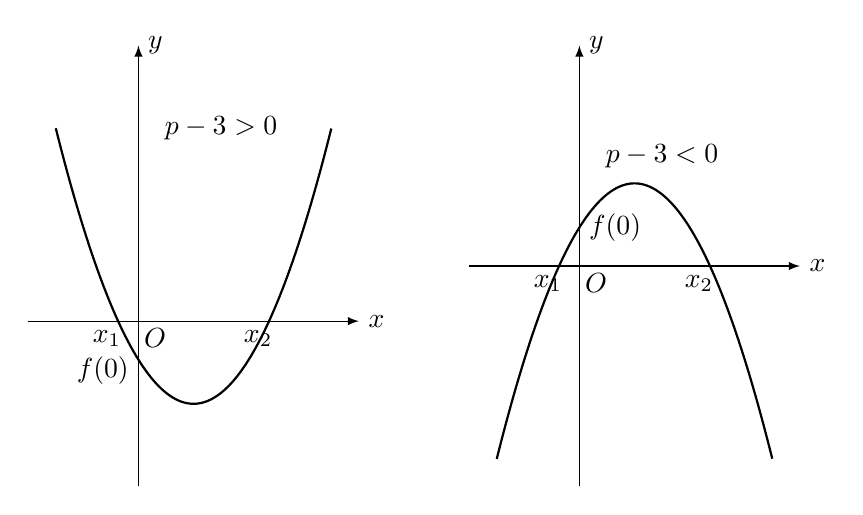
\begin{tikzpicture}[>=latex,scale=.7]
\begin{scope}
\draw[->] (-2,0)--(4,0)node[right]{$x$};
\draw[->] (0,-3)--(0,5)node[right]{$y$};
\draw[domain=-1.5:3.5, samples=100, thick] plot(\x, {(\x-1)*(\x-1)*.8-1.5});
\node at (1.5,3.5){$p-3>0$};
\foreach \x/\xtext in {1.37+1/x_2, -1.37+1/x_1}
{
    \node at (\x-.2,0)[below] {$\xtext$};
}
\node at (.3,-.3){$O$};
\node at (0,-0.9)[left]{$f(0)$};
\end{scope}

\begin{scope}[xshift=8cm, yshift=1cm]
    \draw[->] (-2,0)--(4,0)node[right]{$x$};
\draw[->] (0,-4)--(0,4)node[right]{$y$};
\draw[domain=-1.5:3.5, samples=100, thick] plot(\x, {-(\x-1)*(\x-1)*.8+1.5});
\node at (1.5,2){$p-3<0$};
\foreach \x/\xtext in {1.37+1/x_2, -1.37+1/x_1}
{
    \node at (\x-.2,0)[below] {$\xtext$};
}
\node at (.3,-.3){$O$};
\node at (0,0.7)[right]{$f(0)$};
\end{scope}
\end{tikzpicture}
